\chapter*{Приложение}
\addcontentsline{toc}{chapter}{Приложение}

\begin{figure}[h] % h – размещение "здесь"
    \centering
    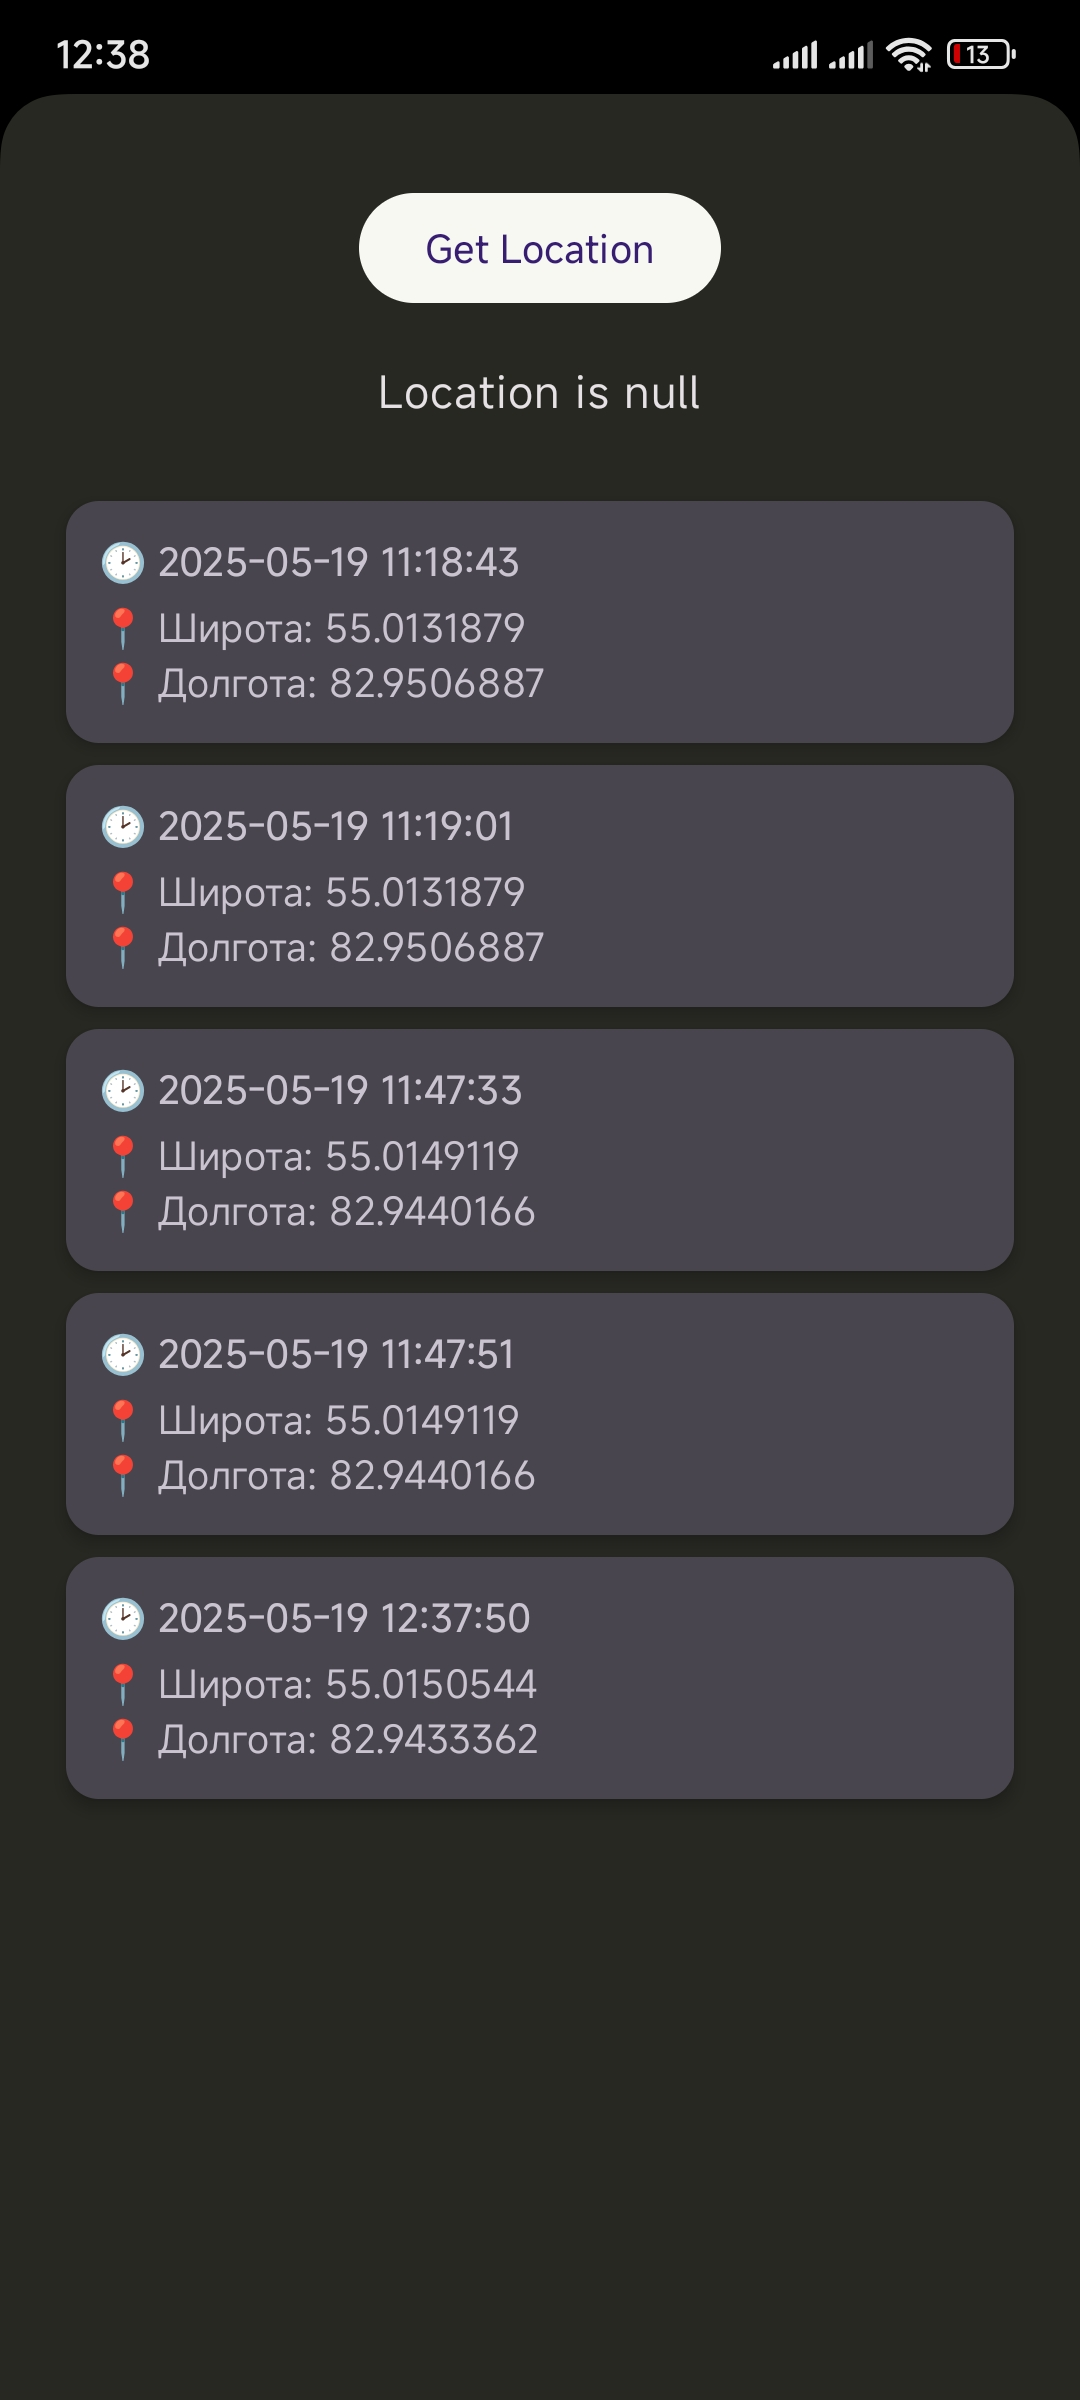
\includegraphics[width=0.5\textwidth]{is null.jpg} % путь и размер
    \caption{Location in null}
    \label{fig:myimage1}
\end{figure}

\begin{figure}[h] % h – размещение "здесь"
    \centering
    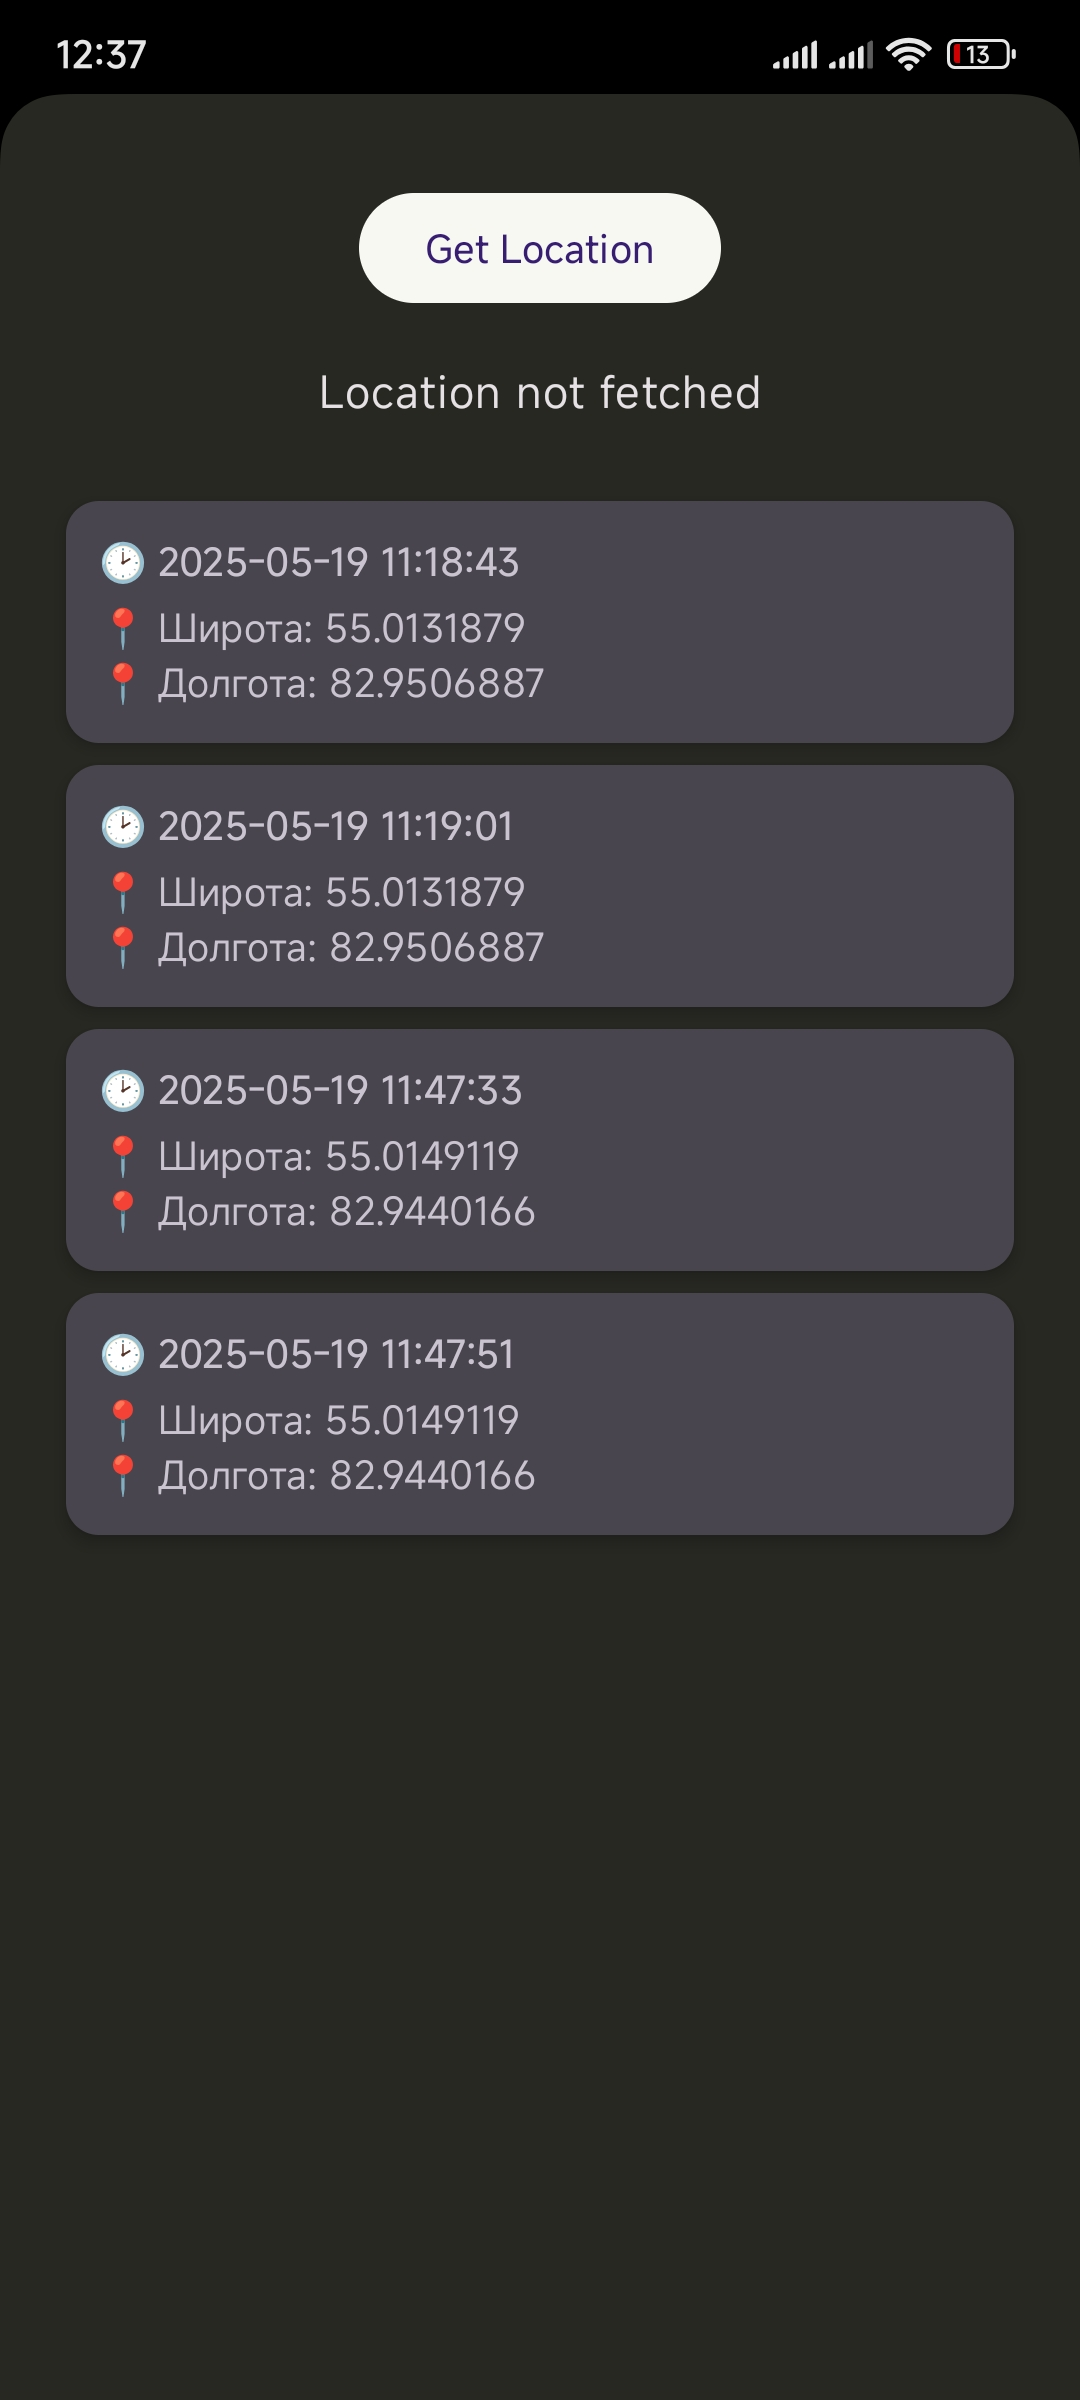
\includegraphics[width=0.5\textwidth]{not_f.jpg} % путь и размер
    \caption{Location not fetched}
    \label{fig:myimage2}
\end{figure}


\begin{figure}[h] % h – размещение "здесь"
    \centering
    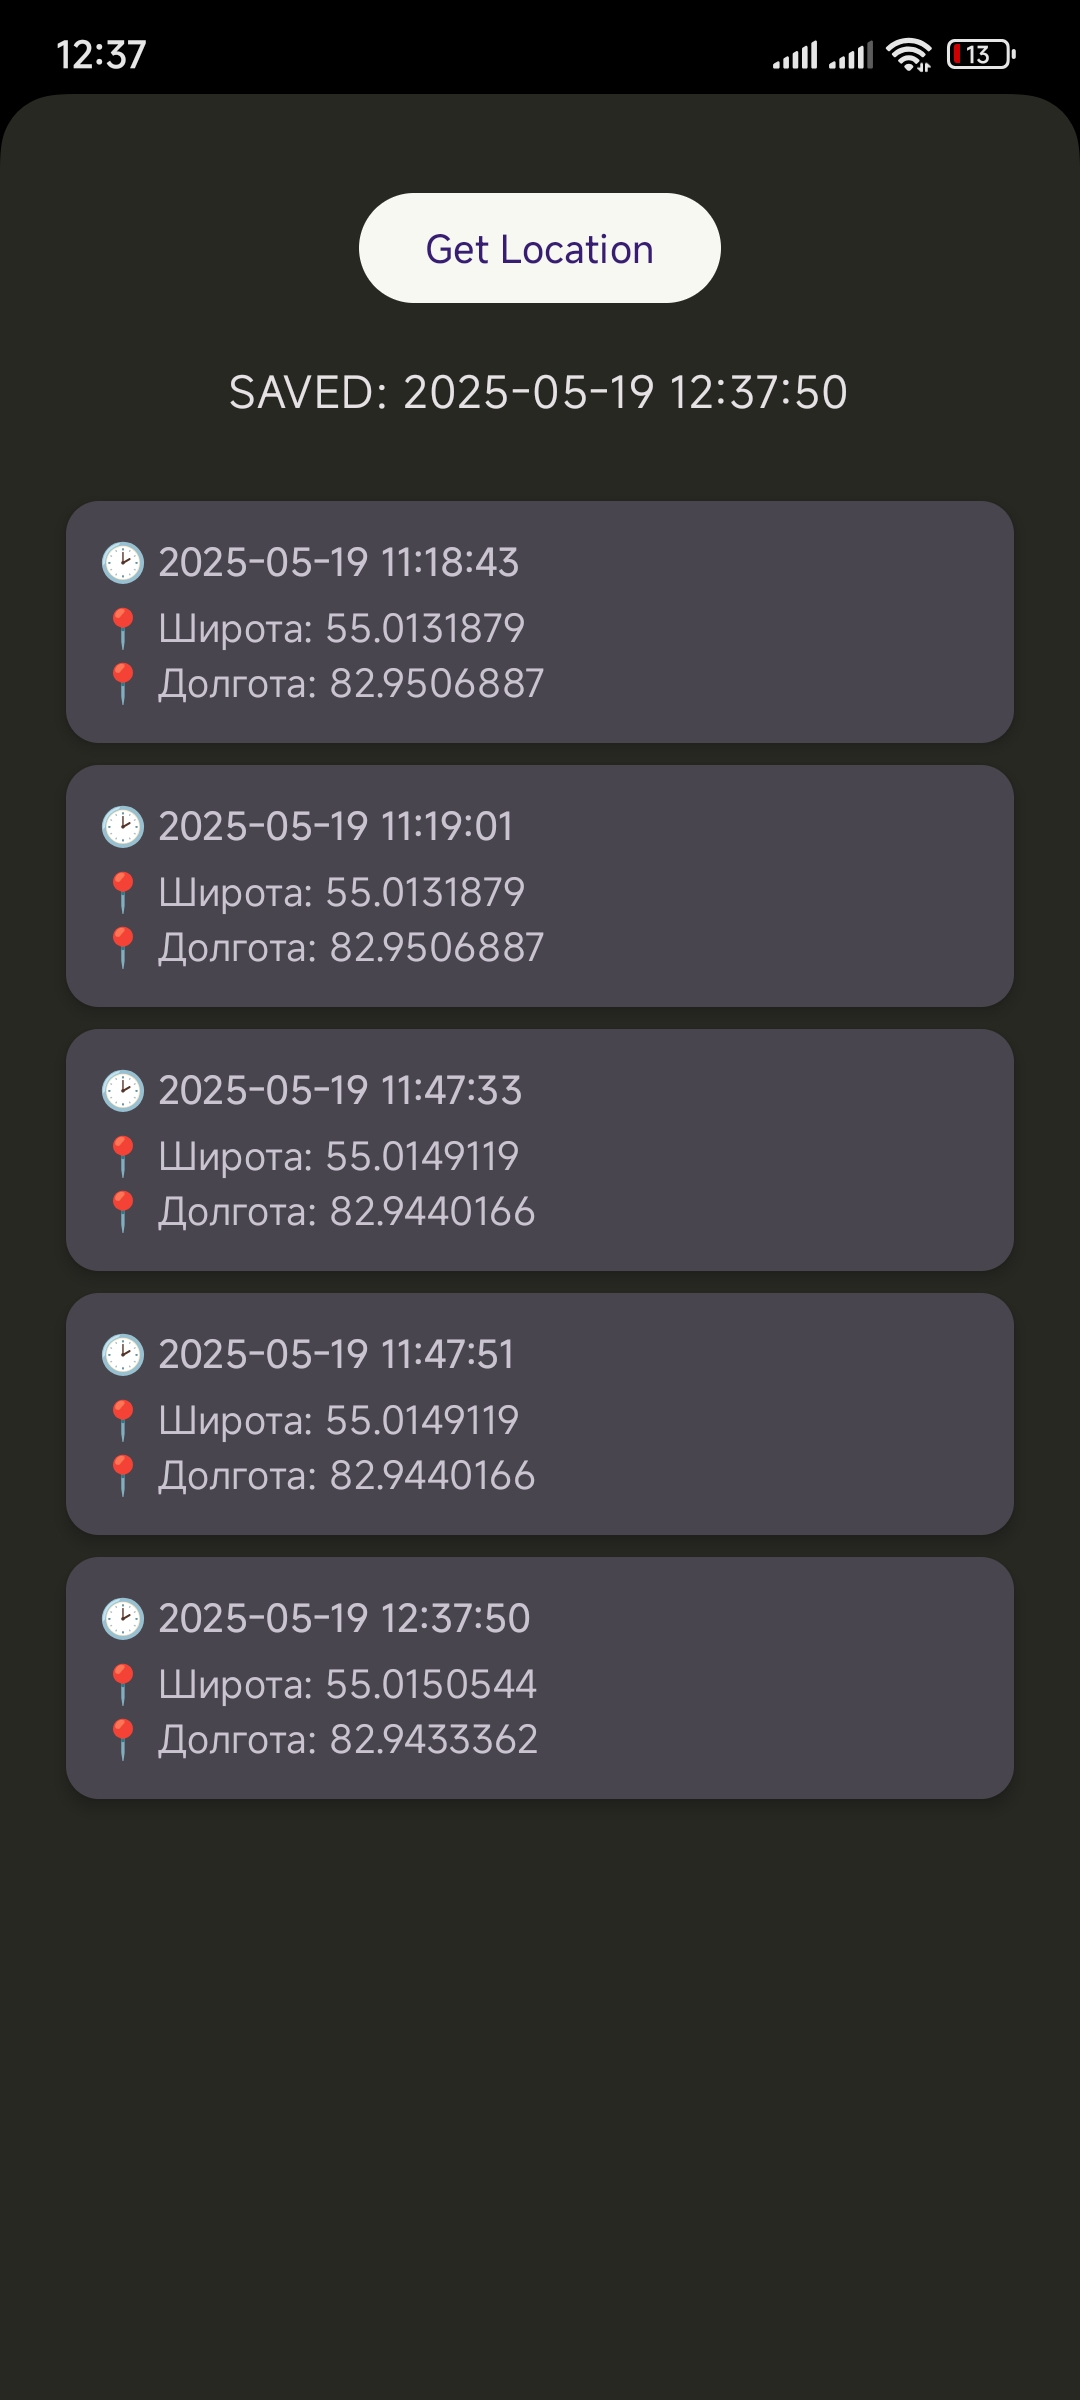
\includegraphics[width=0.5\textwidth]{saved.jpg} % путь и размер
    \caption{Location Saved}
    \label{fig:myimage3}
\end{figure}
